\pagebreak
\section{Wahrscheinlichkeitstheorie}
% Hinweis: Mit \DefReference}{#labelname#} wird angezeigt, welche Definitionen herangezogen wurden, um die Definition aufzubauen.


\subsection{Wahrscheinlichkeitsraum}
Der Wahrscheinlichkeitsraum\footnote{engl. Probability} ist das Kernstück der Wahrscheinlichkeitstheorie. Diese gibt die Werkzeuge, Zufallsexperimente aus der realen Welt zu modellieren.\\

Im Folgenden wird das Konzept von \textit{Ergebnis} uns \textit{Ereignis} konzeptioniert. Mit der gewonnen Ergebnismenge wird das \gls{W.}Maß bestimmt.\footnote{Wenn im Folgenden \gls{W.} als Prefix verwendet wird, ist der Begriff Wahrscheinlichkeit gemeint.}
\begin{Definition}{Wahrscheinlichkeitsraum}
	Sein $\Omega$ eine nichtleere Menge, sei $\SigmaAlgebra$ eine $\sigma$-Algebra auf $\Omega$ und $P$ das \gls{W.}Maß auf $\SigmaAlgebra$, heißt das Tupel $\left(\Omega, \SigmaAlgebra, P\right)$ \textbf{Wahrscheinlichkeitsraum}.
\end{Definition} \footnote{Begrifflichkeit aus der Maß Theorie: \begin{Lemma-Definition}{Maßraum}
	Das Triplet $(\Omega, \SigmaAlgebra, \mathbb{P})$) heißt \textit{Maßraum}, \begin{itemize}
		\item wenn $\Omega$ eine beliebige, nicht leere Menge ist. Diese wird \textit{Grundraum} genannt.
		\item $\SigmaAlgebra$ eine $\sigma-$Algebra über den Grundraum $\Omega$ ist.
		\item $\mathbb{P}$ ein \textit{Maß}, dass auf $\SigmaAlgebra$ definiert ist.
	\end{itemize}
\end{Lemma-Definition}}
Mit den drei Komponenten
Das Konzept der \gls{ZV} wird helfen, einen leichteren Umgang mit dem \gls{W.}Raum zu erhalten. \cite{Mathematik.Arens}, \cite{Stochastik.Henze}

\subsubsection{Ergebnismenge}
Die Menge der möglichen Ergebnisse eines stochastischen Vorgangs wird üblicherweise mit $\Omega$ abgekürzt. Am Anfang einer stochastischen Modellierung ist diese der entscheidenste Schritt, zu definieren, wie diese Menge aussieht. 

\begin{Definition}{Ergebnismenge/raum}
	Die Menge $\Omega$ ist die \textit{Ergebnismenge} oder der \textit{Grundraum} eines Zufallsexperiments und enthält alle möglichen Ergebnisse $\omega$.
\end{Definition}

Dies Definition greift einen naiven Mengenbegriff auf, welcher nur erklärt, ob $\omega\in\Omega$ oder $\omega\notin\Omega$ ist. Diese Eigenschaft scheint in der Theorie trival zu sein, in der Praxis ist es nicht immer klar, ob ein Ergebnis zu einer Grundgesamtheit oder nicht gehört. Ein Beispiel hierfür ist, das \textit{Zufallsvorgang (Experiment): Schwere Unfälle in Berlin}. Ist das Zufallsexperiment ein \textit{Münzwurf}, dann ist der Grundraum leichter zu bestimmen:
\begin{align*}
	\Omega &= \left\lbrace K,Z \right\rbrace \Leerzeichen \text{oder} \\
		&= \left\lbrace Kopf, Zahl \right\rbrace.
\end{align*}

In diesem Fall ist die Mächtigkeit gleich, die genaue Ausprägung von $\omega$ kann jedoch für das gleichgemeinte Zufallsexpermient ungleich sein. Im Falle eines Kartenspiels ist gut zu zeigen, wie unterschiedlich die Grundgesamtheit sogar in ihrer Machtigkeit ausfallen kann: 
\begin{align*}
	\Omega &= \left\lbrace Rot, Schwarz \right\rbrace \Leerzeichen \text{oder} 
	\\
	&= \left\lbrace Rot, Schwarz \right\rbrace \Leerzeichen \text{oder} \\
	&= \left\lbrace RotBild, RotZahl, SchwarzBild, SchwarzZahl  \right\rbrace \Leerzeichen \text{oder}\\
	&= \left\lbrace R2, R3, \dots, SAss \right\rbrace \Leerzeichen \text{oder} \\
	&\text{etc.}
\end{align*}\footnote{Rechtschreibung: Am Ende eines Ganzsatzes setzt man nach Abkürzungen nur einen Punkt. Ausnahmen sind Fragesätze oder Anforderungen.(§ 103 des amtlichen Regelwerks zur deutschen Rechtschreibung)}

Werden $n$ hintereinander durchgeführte Einzelexperimente durchgeführt, können dies als $n-$Tupel eines Gesamtexperiments gesehen werden. Angenommen es liegen zwei Zufallsexperimente vor: 1. Experiment ist ein Münzwurf, das 2. Experiment ist ein Würfelwurf, welche hintereinander durchgeführt werden. Ein adäquater Grundraum für das Gesamtexperiment ist
\begin{align*}
	\Omega_1 \times \Omega_2 = \Menge{(a_1, a_2): a_1 \in \Menge{K,Z}, a_2\in \Menge{1,2, \dots , 6}}
\end{align*}

\subsubsection{Ereignismenge}
Bei stochastischen Vorgängen interessiert oft nur, ob ein Ergebnis $\omega$ zu einer \textit{gewissen Menge von Ergebnissen} gehört. Es wird also eine Menge gesucht, welche alle Fragestellungen an das Zufallsexperiment beantworten kann. Jede Teilmenge von $\Omega$ heißt jetzt ein \textbf{Ereignis}. Diese Teilmengen werden mit Großbuchstaben abgekürzt. \\

Am Beispiel es \textit{Würfel} wird jedes Ergebnis als Ereignis dargestellt: $\Menge{1}, \Menge{2}, \dots, \Menge{6}$. Die Grundmenge $\Omega$ ist ein \textbf{sicheres Ereignis}. Das Ereignis $A$, dass eine gerade Zahl fällt, ist $\Menge{2,4,6}$. Das keine Zahl getroffen wird, wird \textbf{Unmögliches Ereignis} und entspricht $\emptyset$.\\

Um hinreichend komplexe Modelle zu entwickeln, müssen Anforderungen aus der Mengenlehre erfüllt werden. In der Sprache der Mengenlehre, muss die Gesamtheit der Ereignisse eine $\SigmaAlgebra$ bilden, sie \refDefinition{Sigma-Algebra}.


\begin{Definition}{Ereignismenge}
	Sei $\Omega$ eine nichtleere Ergebnismenge, dann heißt das Mengensystem $\SigmaAlgebra$ von Teilmengen auf $\Omega$ eine \textbf{Ergebnismenge}, wenn $\SigmaAlgebra$ eine $\sigma-$Algebra ist (siehe \refDefinition{Sigma-Algebra}).
\end{Definition}\footnote{Begrifflichkeit aus der Maß Theorie: \begin{Lemma-Definition}{Sigma-Algebra}
	Sei $\Omega$ eine nichtleere Obermenge und sei $\SigmaAlgebra$ eine Menge von Teilmengen der Obermenge, dann heißt $\SigmaAlgebra$ eine $\sigma-$Algebra, wenn gilt:
	\begin{itemize}
		\item $\SigmaAlgebra$ enthält die Grundmenge: $\Omega\in \SigmaAlgebra$.
		\item $\SigmaAlgebra$ ist stabil bezüglich der Komplimentbildung: Ist $A\in\SigmaAlgebra$, dann ist auch $A^C\in\SigmaAlgebra$. Dabei ist $A^C$ das Komplement von $A$ bezüglich $\Omega$. 
		\item $\SigmaAlgebra$ ist stabil bezüglich abzählbarer Vereinigungen: Sind $A_i\in \SigmaAlgebra, i\in \N$, so ist auch $\bigcup_{i=1}^{\infty} A_i \in \SigmaAlgebra$.
	\end{itemize}
\end{Lemma-Definition}}

Ist die $\Omega$ eine endliche oder abzählbar unendliche Menge, so die größte $\sigma-$Algebra die aufgespannte Potenzmenge. Die kleinste ist $\Menge{\emptyset, \Omega}$.\\

Beim \textit{Wurf} einer Münze ist $\Omega = \Menge{K,Z}$. Die erzeugte von $\Omega$ erzeugenden $\sigma-$Algebra die Potenzmenge $\Menge{\emptyset, \Menge{K}, \Menge{Z}, \Menge{K,Z}}$. 

\subsubsection{Wahrscheinlichkeitsmaß}
Der Begriff der Wahrscheinlichkeit ist inhaltlich leer. Dieser beruht auf das axiomatische Fundamente von \textit{Kolmogorov}. Dies lässt ein großen Spielraum für die Interpretationen und Berechnungen offen. Solang die Axiomen eingehalten werden, kann eine Wahrscheinlichkeit als relative Häufigkeit, Grenzwert von Häufigkeiten als Expertenmeinung oder etc. verstanden werden.

\begin{Definition}{Drei Axiome von Kolmogorov/ Wahrscheinlichkeitsmaß}
	Sei $\Omega$ eine Obermenge, sei $\SigmaAlgebra$ eine $\sigma-$Algebra von $\Omega$, heißt die Abbildung $P$ von $\SigmaAlgebra$ nach $\R$ \textbf{Wahrscheinlichkeitsverteilung} oder \textbf{Wahrscheinlichkeitsmaß} von $\Omega$ (genauer: auf den Teilmengen von $\Omega$), wenn für $P$ gilt:
	\begin{itemize}
		\item Axiom Nichtnegativität und Normiertheit: $\forall A\in \SigmaAlgebra: 0\leq P(A) \leq 1$
		\item Axiom Normiertheit: $P(\Omega) = 1$
		\item Axiom $\sigma$-Additivität: Für jede abzählbare Folge von disjunkten Mengen $A_i\in \SigmaAlgebra$ gilt
		\begin{align*}
			P\left( \bigcup_{i=1}^{\infty}A_i \right) = \sum_{i=1}^{\infty} P(A_i).
		\end{align*}
	Der Wert von $P(A)$ heißt Wahrscheinlichkeit.
	\end{itemize}
\end{Definition} \footnote{Alternative Beschreibung aus der Maß Theorie: \begin{Lemma-Definition}{Maß}
	Es sein $\SigmaAlgebra$ eine $\sigma-$Algebra einer nichtleeren Grundmenge $\Omega$. Eine Abbildung $f:\SigmaAlgebra\rightarrow [0,\infty]$ heißt \textit{Maß} auf $\SigmaAlgebra$, wenn die beiden Bedingungen erfüllt sind:
	\begin{itemize}
		\item $f(\emptyset)=0$
		\item $\sigma-$Algebra Additivität.
	\end{itemize}
\end{Lemma-Definition}}
Das \gls{W.}Maß kann somit als Abbildung in $[0,1]$ verstanden werden.\\

Für den Wurf eines Münze würde für $\Omega = \Menge{K,Z}$ das \gls{W.}Maß wie folgt aussehen:
\begin{align*}
	P: \SigmaAlgebra \rightarrow [0,1],
	A \mapsto P(A) = \begin{cases}
		P(\Menge{K}) & = 0,5\\
		P(\Menge{Z}) & = 0,5\\
		P(\Menge{Z,K}) & = 1\\
		P(\emptyset) & = 0\\
	\end{cases}
\end{align*}
Nicht immer wird eine Vorschrift für jede Menge $A\in\SigmaAlgebra$ definiert oder auch der das Ergebnis richtig definiert. 
\begin{itemize}
	\item Sei $\Omega = {1,2, \dots, 6}$ die Ergebnismenge für einen Würfelwurf. Es kann beobachtet werden, dass $P(i) = \frac{1}{6} \forall i \in \Omega$ angegeben wird. Das \gls{W.}Maß nimmt jedoch nur Mengen auf, weshalb es richt wäre $P(\Menge{i})$ zu notieren. 
	\item Selbst wenn $P(\Menge{i})$ notiert wird, wird durch die $\sigma-$Additivität $P(\Menge{2,4,6}) = \frac{1}{6} + \frac{1}{6} + \frac{1}{6} = \frac{3}{6}$ hergeleitet.
	\item Wenn bei wiederholten Experimenten \textit{Totale Unabhängigkeit} vorliegt, kann bei einem dreimaligen Münzwurf $P(\Menge{KZK}) = P(\Menge{K})P(\Menge{Z})P(\Menge{K})$ mit $\left(\frac{1}{2}\right)^3$.
\end{itemize}

\subsection{Zufallsvariable und Verteilungen} \label{sec: Zufallsvariable und Verteilungen}
Das Konzept der \gls{ZV} % auschreiben
dient des leichteren Umgangs mit dem \gls{W.}Raum. Rechnungen und weitere aufgesetzten Konzepte werden nicht mehr in einem abstrakten Raum $\Omega$ bestimmt, sondern im $\R^1$ oder auch bei mehrdimensionale \gls{ZV} der $\R^k$ mit $k\in \N$. 

\subsubsection{Herleitung}
Schlussendlich erzeugt die Zufallsvariable einen neuen \gls{W.}Raum, welcher auf einem Erzeugerraum $(\Omega, \SigmaAlgebra, P)$ definiert wird. Dabei werden unter gewissen Bedingungen Eigenschaften dieses Erzeugerraums auf die Zufallsvariable übertragen, so auch die Bildung des neuen \gls{W.}Maß $P_X$.
\paragraph{Bemerkung}
\begin{itemize}
	\item \gls{ZV} werden mit Großbuchstaben aus dem hinteren Bereich des Alphabetes notiert: $X,Z,W,$ etc.
	\item Es gibt auch anderen Begrifflichkeiten für \gls{ZV}. Vom Prinzip handelt sich sich bei einer \gls{ZV} nicht um eine Variable sondern um eine Abbildung. Weil \gls{ZV} jedoch im Verbindung mit dem \gls{W.}Raum betrachtet und weiterverarbeitet werden, kommt diese Bezeichnung zustanden. Realisationen einer \gls{ZV} werden nie einzeln betrachtet, sie werden immer in der ein oder anderen Weise in Abhängigkeit ihres zugehörigen \gls{W.}Maß betrachtet. Aus diesem Zusammenhang leitet sich auch der Begriff des Zufalls ab, für die Interpretation einer Realisierung kommt immer in Frage, wie wahrscheinlich das eintreten dieses Event ($\SigmaAlgebra$) ist. Der Zufall entscheidet über die Verteilung und gibt so eine variable Größe wieder. Daher kommt auch der andere Name \textit{Zufallsgröße} zustande. Betrachtet man höherdimensionale \gls{ZV} spricht man von \textit{Zufallsvektoren}. 
\end{itemize}

\paragraph{Definition}
In der einfachsten Form ist eine \gls{ZV} eine Abbildung, welche aus $\Omega$ eine \gls{W.}Raums c auf $\R$ abbildet. Diese Abbildung muss nicht bijektiv oder injektiv sein. Somit könnte gelten
\begin{Definition}{Zufallsvariable}
	Sei $(\Omega, \SigmaAlgebra, P)$ ein \gls{W.}Raum. Die Abbildung
	\begin{align*}
		X: \Omega \rightarrow \R
	\end{align*}
	heißt \textit{Zufallsvariable}.
\end{Definition}

\textit{Allgemeiner Vermerk: Eine mathematische Definition kann auf verschiedenen Weise beschreiben werden. Welche Konzepte wann angebracht werden, kann aus den verschiedensten Gründen erfolgen. Schlussendlich besteht das Ziel, ein Problem lösen zu können. 
Bei dem Konzept der Zufallsvariable gilt das gleiche. Es können Element der Maßtheorie in die Definition gezogen werden. Ebenso können Bestandteile des \gls{W.}Maß $P_X$ vorgezogen werden, und an die Definition des Zufallsvariablen angefügt werden. Bsp.:}
\begin{itemize}
	\item \begin{Lemma-Definition}{Alternative Definition I der Zufallsvariable}
		Sei $(\Omega, \SigmaAlgebra, P)$ ein \gls{W.}Raum. Die Abbildung
		\begin{align*}
			X: \Omega \rightarrow \R
		\end{align*}
		heißt \textbf{Zufallsvariable}, wenn bei der das vollständige Urbild $X^{-1}(B)$ jeder Borel-Menge $B\in\SigmaAlgebraIndividuel{B}$ ein Element von $\SigmaAlgebra$ ist.
	\end{Lemma-Definition}
	\item \begin{Lemma-Definition}{Alternative Definition II der Zufallsvariable}
		Sei $(\Omega, \SigmaAlgebra, P)$ ein \gls{W.}Raum und $(\Omega_2, \SigmaAlgebra_2)$ ein Messraum, so heißt die Abbildung
		\begin{align*}
			X: \Omega \rightarrow \Omega_2
		\end{align*}
		\textbf{Zufallsvariable}. Ist $\Omega_2=\R^k$, so wird $X$ als $k-$\textit{dimensionale reelle Zufallsvariable} und im Fall $k=1$ als \textit{reelle Zufallsvariable} bezeichnet.
	\end{Lemma-Definition}
\end{itemize}

Die \gls{ZV} ist eine Vorschrift, welche jedem Ergebnis $\omega$ eines stochachstischen Vorgang eine Wert $X(\omega$) zu weißt. Dies Werte werden als \textit{Realisationen von} $X$ bezeichnet. Ebenso können sie als Messung einer stochastischen Experiment interpretiert werden.
 
\paragraph{Borel Sigma Algebra}
Um das \gls{W.}Maß $P_X$ zu definieren, wird die \SigmaAlgebraText auf $\R$ benötigt. Für abzählbare Mengen $\Omega$ war die größte \SigmaAlgebraText die Potenzmenge \Potenzmenge$(\Omega)$. Für $\R$ ist es die Borel-\SigmaAlgebraText.\footnote{Referenz: \href{https://de.wikipedia.org/wiki/Messbare{\_}Funktion}{Wikipedia/MessbareFunktion}}
\begin{Definition}{Borelsche Sigma-Algebra}
	Sei $\Omega$ eine topologischer Raum und $O$ das System der offenen Teilmengen von $\Omega$. Dann heißt
	\begin{align}
		\SigmaAlgebraIndividuel{\Omega} := \sigma(O)
	\end{align}
	die \textit{Borelsche} \SigmaAlgebraText über $\Omega$. Ihre Elemente $B\in\SigmaAlgebraIndividuel{B}$ heißen \textit{Borelsche-Mengen} oder \textit{Borel-Mengen}. Im Fall $\Omega=\R^k$ setzen wir $\SigmaAlgebraIndividuel{B}^k:=\SigmaAlgebraIndividuel{\R^k}$, im Fall $k=1$ ist $\SigmaAlgebraIndividuel{B}:=\SigmaAlgebraIndividuel{\R^1}$.
\end{Definition}

\paragraph{Bemerkung}
\begin{itemize}
	\item Borel-\SigmaAlgebraText wird über einen Erzeuger $E$ definiert und wird nicht direkt von $\Omega$. Beispiel für $\Omega=\R$ sind
	\begin{align*}
		E_1 & = \Menge{(-\infty, a]: a\in \R},
		E_2 & = \Menge{(-\infty, a): a\in \R},
		E_3 & = \Menge{(a, b) \subset \R:  a \leq b}, \text{etc.}
	\end{align*}
	\item Die \textit{Borel-}\SigmaAlgebraText ist die kleinste \SigmaAlgebraText die alle Teilmengen von $\Omega$ besitzt.
	\item Für den weiteren Verlauf wird nicht weiter darauf eingegangen, welcher Erzeuger die \textit{Borel}-\SigmaAlgebraText erzeugt.
\end{itemize}

\paragraph{Verteilung einer Zufallsvariable}
Es besteht folgendes Problem. Wie kann sicherstellt werden, dass die Eigenschaften der Wahrscheinlichkeitsverteilung des Erzeugerraums $\WRaum$ erhalten bleiben oder sich in gewisserweise übertragen. Hierfür wird für $X$ die \textit{Messbarkeitseingeschaft} verlangt. \\

Diese besagt im Kontext der Maß Theorie
\begin{Lemma-Definition}{Messbarkeitseigenschaft}
	Eine Abbildung $f$ heißt \textit{messbar}, wenn das Urbild jeder Menge $B\in\SigmaAlgebraIndividuel{B}$ unter $f$ ein Element aus \SigmaAlgebra ist.
\end{Lemma-Definition}
Formaler bedeutet diese
\begin{align}
	f^{-1}(B)\in \SigmaAlgebra\Leerzeichen \forall B\in \SigmaAlgebraIndividuel{B}
\end{align}
\paragraph{Bemerkung Messbarkeitseigenschaft}
\begin{itemize}
	\item Der Ausdruck $f^{-1}(B)$ bezeichnet dabei keine Abbildung, sondern die Urbildmenge.
	\item Alternative Schreibweisen sind $\Menge{\omega\in \Omega: f(\omega)=x}\in \SigmaAlgebra$ für $\forall x\in \R$.
	\item Diese Anforderung stellt für die Definition oder Konzeption einer Zufallsvariable sicher, dass das Urbild eines Ereignis in $\SigmaAlgebraIndividuel{B}$ auch ein Ereignis in \SigmaAlgebra unter $\Omega$ ist.
\end{itemize}
Hintergrund ist, diese Mengengebilde $\Menge{\omega \in \Omega: X(\omega) = x} \in \SigmaAlgebra$ wird für das \gls{W.}Maß $P_X$ benötigt. Denn im Bezug auf die \gls{ZV} $X$ beleibt die Frage bestehen, wie kann die Wahrscheinlichkeitsverteilung von $\Omega$ über $X$ auf $P_X$ übertragen. Die Antwort: \refDefinition{Messbarkeitseigenschaft}.
Damit diese Definition der \textit{Verteilung von} $X$ greift, muss zur Definition einer Zufallsvariable die Messbarkeitseigenschaft (messbar) ergänzt werden.
\begin{Definition}{Zufallsvariable und Messbarkeitseigenschaft}
	Sei $(\Omega, \SigmaAlgebra, P)$ ein \gls{W.}Raum und $(\R, \SigmaAlgebraIndividuel{B})$ ein Messraum, so heißt die die $\Omega-\R$-messbare Abbildung
	\begin{align*}
		X: \Omega \rightarrow \R
	\end{align*}
	\textbf{Zufallsvariable}.
\end{Definition}

\begin{Definition}{Verteilung einer Zufallsvariable/ Wahrscheinlichkeitsfunktion}
	Sei \WRaum und $(\R, \SigmaAlgebraIndividuel{B})$ ein Messraum und $X: \Omega \rightarrow \SigmaAlgebraIndividuel{B}$ eine Zufallsvariable, so heißt das Bildmaß
	\begin{align*}
		P_X(B):=P(X^{-1}(B))
	\end{align*}
	Verteilung von $X$ oder auch \textit{Wahrscheinlichkeitsverteilung} im diskreten oder \textit{Dichtefunktion} im stetigen Fall.
\end{Definition}
\begin{figure}[H]
	\centering
	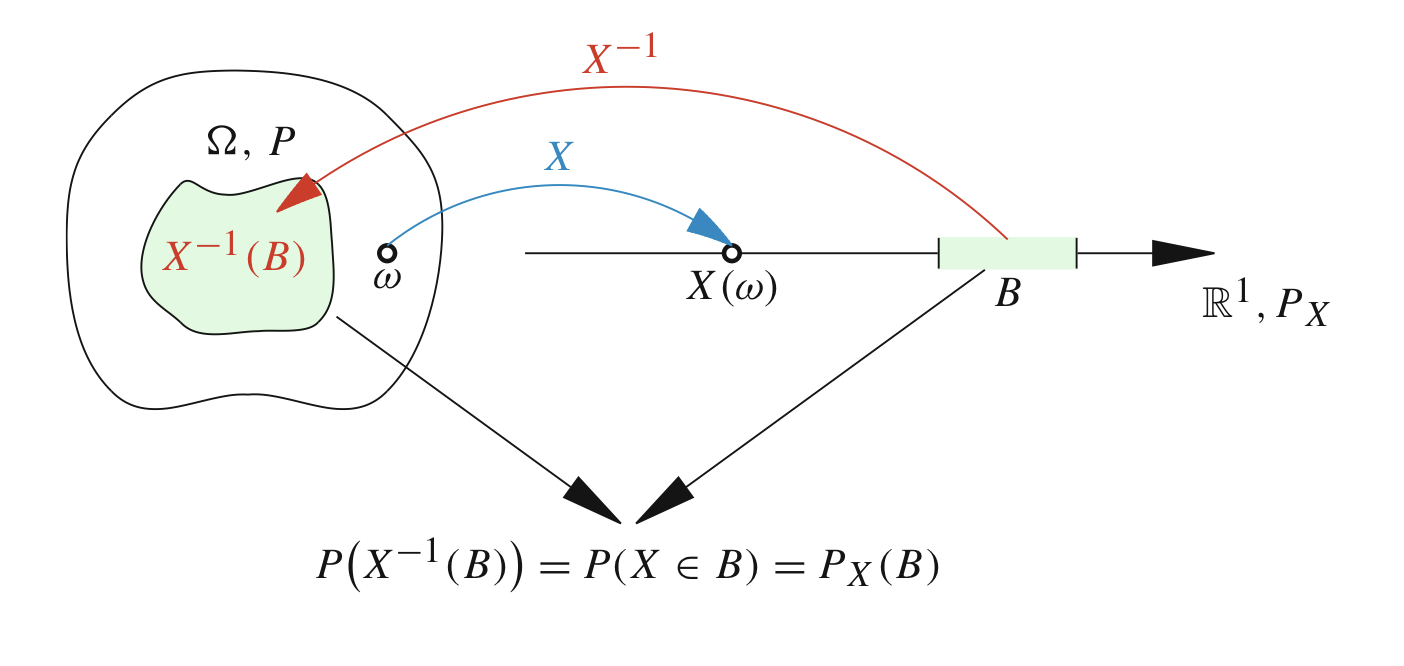
\includegraphics[scale = 0.4]{attachment/chapter_9/Scc002}
	\caption{Die Zufallsvariable $X$ bildet $\Omega$ in $\R$ ab und überträgt die Wahrscheinlichkeiten der Ereignisse}
\end{figure}

\begin{itemize}
	\item Wegen der \textit{Messbarkeitseigenschaft} ist das Bildmaß $P_X$ auf $\Omega$ gilt $P_X(\Menge{\R}) = P(\Omega) = 1$
	\item Eigenschaften der Verteilung $P_X$ werden als Eigenschaften von $X$ deklariert. Z. B.: Wenn $P_X$ diskret ist, ist auch $X$ diskret. Wenn $P_X = \Normalverteilung{\mu, \sigma^2}$, so wird 
	\begin{align*}
		X \sim \Normalverteilung{\mu, \sigma^2}
	\end{align*}
	notiert.  Das Symbole $\sim$ wird nicht einheitlich ausgedrückt. Für den weiterem Umgang, wird hier angenommen, dass es für \textit{verteilt nach} steht.
	\item Andere Schreibweisen für das \gls{W.}Maß $P_X$ sind
	\begin{align*}
		P(X\in B) &:= P_X(B) := P(\Menge{\omega \in \Omega: X(\omega)\in B}),\\
		P(X = x) &:= P_X({x}) := P(\Menge{\omega \in \Omega: X(\omega) = x}),\\
		P(X \leq x) & := P_X((-\infty, x]) := P(\Menge{\omega \in \Omega: X(\omega) <= x}),
		\text{etc.}
	\end{align*}
\end{itemize}
\footnote{Kommt die Frage auf, ist der Ausdruck $P(X\leq x)$ überhaupt möglich, wenn nicht sichergestellt werden kann, ob die Zufallsvariable mindestens eine ordinale Skalierung besitzt? Die Antwort: Ja. Das \gls{W.}Maß gibt nur wieder, wie die Verteilung von $X$ aussieht und die Realisationen in $\R$ zu verwerten sind. Dabei gibt es eine gegeben Ordnung in $\R$. Ob diese Sinn ergibt, hängt von der Skala ab. Dies ist Thema im Kapitel \textit{Deskriptive Statistik}.}

Auf der Verteilung von $X$ aufbauend wird die \textit{Verteilungfunktion von X} definiert.
\begin{Definition}{Verteilungsfunktion von X}
	Ist $X$ eine Zufallsvarialbe auf einen WS-Raum $(\Omega, \mathcal{F}, \mathbb{P})$, so heißt die durch 
	\begin{align*}
		F_X(x):= 	\mathbb{P}(X\leq x), x\in \R
	\end{align*}
	definierte Abbildung $F_X: \R \rightarrow [0,1]$ die \textit{Verteilungsfunktion von} $X$. Diese besitzt die Eigenschaft \textit{monoton wachsend}, \textit{rechtsseitig stetig} und $F_X$ kommt von 0 und geht nach $1$.
\end{Definition}

\subsubsection{Eigenschaften und Besonderheiten}
\paragraph{Diskret ZV}
Handelt es sich bei $X$ um eine stetige oder diskrete \gls{ZV} ist damit die \textit{Wahrscheinlichkeitsfunktion} oder \textit{Dichtefunktion} gemeint. Dies Eigenschaft wird sprachlich auf die Abbildung $X$ gemünzt.\\

\begin{Definition}{Diskrete Wahrscheinlichkeitsverteilung einer diskreten zufälligen Variablen}
	Eine \textit{diskrete} Zufallsvariable $X$ besitzt endlich oder abzählbar unendlich viele Realisationen $x_i$, die mit Wahrscheinlichkeiten 
	\begin{align*}
		p_i = P(X=x_i) > 0
	\end{align*}
	angenommen werden. Für $x_i$ gilt
	\begin{align*}
		\sum_{i=1}^{\infty} P(X=x_i) = 1.
	\end{align*}
	Die Angaben aller $p_i$ heißen \textit{Wahrscheinlichkeitsverteilung von} $X$.
\end{Definition}

\paragraph{Verteilung im Erzeugerraum bekannt}
Im Fall, dass $\Omega$ sich nicht bestimmen lässt oder $P$ sich nicht abbilden lässt, ist das Wissen gut, dass für den \gls{W.}Raum von $X$ es ausreicht, wenn die $F_X$ bekannt ist. Dies erlaubt, dass direkt im aufgespannten Raum zu bleiben.

\paragraph{Kanonische Konstruktion}
Lässt sich $\Omega$ nicht definieren oder ist zu kompliziert darzustellen. Kann für $\Omega$ gleich mit $\R$ gesetzt werden. Für $\SigmaAlgebra$ wird $\SigmaAlgebraIndividuel{B}$ gesetzt. Für die Abbildung von $\Omega$ nach $\R$ wird die Indentität gewählt.\\

Die Art des Aufbaues des neuen \gls{W.}Raums nennt sich \textbf{Kanonische Konstruktion} bei $X(x):= x$ ist. Dies ist nicht untypisch in der Statistik, dass der \gls{W.}Raum \WRaum in den Hintergrund gerät.

\paragraph{Verteilungen}
Verteilungen wie Bernoulli, Poison, Normalverteilt, etc. bestimmen sich aus den gegeben Parametern des zu Grunde liegenden Sachverhalt der \gls{W.}Raums.

\paragraph{Nicht messbare Abbildung}
Sei $X=Y=\Menge{1,2}$ und $\SigmaAlgebra = \Menge{\emptyset, X}$ (Kleinste $\sigma-$Algebra) und $\SigmaAlgebraIndividuel{B} = \Potenzmenge(X)$.\\

Die Frage: Ist $\SigmaAlgebra-\SigmaAlgebraIndividuel{B}-f$ messbar, wenn $f(1):=2$ und $f(2):=1$ definiert ist?\\

Antwort: Nein, die Abbildung ist nicht messbar. 
Für $f^{-1}(\Menge{2})$ müsste das Ereignis $\Menge{1}$ in $\SigmaAlgebra$ liegen.\footnote{Referenz: \href{https://matheraum.de/forum/nicht{\_}messbare{\_}Funktion/t725285}{Matheraum/nicht messbare Funktion}}\\


Hinweis: Für \textit{messbare} \gls{ZV} wird im diskreten Fall die Potenzmenge für $\Omega$ herangezogen.

	
\subsubsection{Beispiele}
\paragraph{Beispiel zweifacher Würfelwurf}
Der Erzeugerraum wird für den stochastischen zweifachen Würfelwurf
\begin{align*}
	\Omega = \Menge{1,2,3,4,5,6}^2 = \Menge{\omega = (\omega_i)_{i\in \Menge{1,2}}: \omega_i \in \Menge{1,2,3,4,5,6}}
\end{align*}
Ein Ereignis $A = \Menge{2,4,6}$ könnte die Menge der geraden Zahlen sein. Bei der Zufallsvariable $X$ interessiert \textit{Die Summe der Augenzahlen}. Die Abbildungsvorschrift sieht dabei wie folgt aus
\begin{align*}
	X = \begin{cases}
		1 &,\, \text{wenn}\, (1,1)\\
		2 &,\, \text{wenn}\, (1,2)\\
		\vdots & \vdots \\
		36 &\, \text{wenn} (6,6)
	\end{cases}
\end{align*}
Das \gls{W.}Maß $P$ auf $\Omega$ definiert sich gleichverteilt: $P(\Menge{\omega}) = \frac{1}{36}$. Für $P_X$ leitet sich aus der \refDefinition{Messbarkeitseigenschaft} ab, die Kombinationen von $\omega$ welche die Summenzahl $x_i$ ergeben, werden aufaddiert. Als Beispiel: 
\begin{align*}
	&X = 4 - \text{Summe 4 der Augenzahlen zweier Würfel}\\
	&\rightarrow P_X(\Menge{X=4}) = P(\Menge{(1,3), (2,2), (3,1)}) \\
	&= \frac{1}{36} + \frac{1}{36} + \frac{1}{36} + \frac{1}{36}\\
	&= \frac{4}{36}
\end{align*}

\paragraph{Beispiel Plurale Informationen}
Gegeben sei eine Population von Menschen mit $\Omega = \Menge{\text{Silvia}, \text{Manfred}, \dots}$ von diesen können Informationen (Plural) gezogen werden. 
\begin{itemize}
	\item Körpergewicht $\R_{>}$. Diese genau \textit{Wahrscheinlichkeitsverteilung} $P_X$ ergibt sich aus den konkreten Urbilder zu jeden Wert von $x$.
	\item Die Information Parteizugehörigkeit kann ebenfalls als Zufallsvariable abgebildet werden. Die Parteien werden einer belieben Zahl zugeordnet. Je nach dem wie in der Population die Personen den Parteien zugeordnet sind, bestimmen die Urbilder über der Verteilung der \gls{ZV}.
\end{itemize}

\subsubsection{Momente einer Zufallsvariable}
Momente von \gls{ZV} sind Parameter/Kenngrößen der Deskriptiven Statistik. Das Konzept des Moment wird auch genutzt in der Inferenz Statistik, um Schätzer zu konstruieren. \\
Die bekanntesten Momente sind Erwartungswert, Varianz, Schiefe und Wölbung. Es gilt, eine Verteilung einer \gls{ZV} ist eindeutig bestimmt, durch die Angabe aller Momente, falls diese existieren und die momentenerzeugenden Funktionen konvergieren.\\


\paragraph{k-tes theoretische Moment}
Sei $X$ eine Zufallsvariable und $k$ eine natürliche Zahl. Man bezeichne das $k-te$ Moment von $X$ als Erwartungswert der $k-ten$ Potenz von $X$:
\begin{align}
	m_k := \Erwartungswert{X^k}
\end{align}

Das $1-$ Moment von $X$ ist der \textbf{Erwartungswert} $\mu$.

\paragraph{k-tes absolutes Moment}
Das absoluten Moment ist erhält die Ergänzung
\begin{align}
	m_k^a := \Erwartungswert{\lvert X \rvert^k}
\end{align}

\paragraph{k-tes zentrales Momente}

Beim $k-ten$ zentralen Moment wird der Erwartungswert von $X$ von $X$ abgezogen:
\begin{align}
	\mu_k := \Erwartungswert{(X - \mu_1)^k}.
\end{align}
Das zweite zentrale Moment ist die Varianz $\sigma^2 := \mu_2$. Bei dritten spricht man von der Schiefe und vom vierten von der Wölbung. In beiden Fällen wird das Moment noch mit der Standardabweichung $\sigma$ normiert:

\begin{align}
	\mu_{3/4}^s := \Erwartungswert{\left(\frac{X- \mu}{\sigma}\right)^{3/4}}
\end{align}


\paragraph{Beispiel stetiges und diskrete Zufallsvariable} \label{paragraph: Erwartungswert} 
Am Beispiel des Erwartungswertes wird das Moment für eine stetige und diskrete \gls{ZV} aufgezeigt.
\begin{Definition}{Erwartungswert (stetig)}
Ist $X: \Omega \rightarrow \R$ eine quasiintegrierbare reelle Zufallsvariable, so heißt
\begin{align*}
	\Erwartungswert{X} := \int XdP = \int xd P_X(x)
\end{align*}
der Erwartungswert von $X$.
\end{Definition}

Ist $X$ diskret, so definiert sich der Erwartungswert wie folgt:
\begin{Definition}{Erwartungswert (Diskret)}
	Für eine reele Zufallsvariable $X$ auf eine endlichen \gls{W.}Raum \WRaum heißt
	\begin{align*}
		\Erwartungswert{X}:= \Erwartungswert{X}_P := \sum_{\omega\in\Omega} X(\omega)P_X(\Menge{\omega})
	\end{align*}
	der Erwartungswert von $X$.
\end{Definition}
Das $P_X(\Menge{\omega})$ angegeben wurde, bezieht sich darauf, dass zu jedem $\omega$ es unterschiedliche oder auch gleiche $x$ abgebildet werden können.\footnote{
	Quelle: \href{
		https://de.wikipedia.org/wiki/Moment{\_}(Stochastik)
	}{
		Moment(Wiki))
	}.
}
\subsection{Statistisches Modell}

Wie in der Einleitung für Stochastik erwähnt, die Kategorisierung in \textit{Deskripter/ \gls{EDA}} und Inferenzstatistik muss sich nicht immer in den Methoden unterscheiden. Oftmals werden die gleichen Sachverhalten etwas modifiziert, um die Fragestellung beantworten zu können. Zum Beispiel auch hier, beim \gls{SM}. Das \gls{SM} in der theoretischen Form beschreibt die Variation des \WRaum durch die Para- und Nichtparametisierung der Verteilungsfunktion. Wenn im Folgenden vom Stichprobenraum und angepasste Parameterräumen gesprochen wird dann wird das Werkzeug des \gls{SM}s in Richtung Inferenz Statistik getrieben.


\paragraph{Motivation}
Das \gls{SM} vereinfacht oder passt das vorherige Verständnis eines \gls{W.}Raum an.
Für die Modellierung eines \gls{W.}Raum wird eine konkrete \gls{W.}Verteilung/ \gls{W.}Maß festgelegt. Dies wird im \gls{SM} durch eine Tupel von \gls{W.}Maße ersetzt. Dieses Tupel ist 
\begin{align*}
(P^X_{\vartheta})_{\vartheta\in\Theta}\Leerzeichen - \Leerzeichen \text{die parametrische Familie möglicher Verteilungen von}\Leerzeichen X.
\end{align*}

Es wird angenommen, dass die \textit{wahre} Verteilung zu diesem Tupel gehört.
Im Allgemeinen wird von einem \textit{Parameter} gesprochen. Dieser kann auch mehrdimensional sein, wie auch bei der Normalverteilung mit $(\mu, \sigma^2)$. Ebenso wird im Allgemeinen von einer \gls{ZV} gesprochen, wenn auch hier eine mehrdimensional \gls{ZV} vorliegt.\\

\begin{Lemma-Definition}{Parameterraum}
	Die Menge aller möglichen Werte des Parameter $\vartheta$ wird \textit{Parameterraum} $\varTheta$ genannt.\\
\end{Lemma-Definition}
Ein Parameter $\vartheta$ kann auch mehrdimensional sein.\\

Der Grundgesamtheit liegt ein unbekannter aber fester Parameter $\vartheta\in\varTheta$ zugrunde - Beim \gls{SM} ist der Parameter auf die Verteilungsfunktion bezogen. Im Regressionsmodell beziehen sich die Parameter auf die Beziehungen zwischen den \gls{ZV}. Dieser Parameter wird aus der Stichprobe geschätzt. \textbf{Bsp.:} Sei $X\sim\Normalverteilung{\mu, \sigma^2}$ wird mit Hilfe der Stichproben  $\vartheta = (\mu, \sigma^2)\in \varTheta \subset \R\times\R^+$ versucht zuschätzen.\\

%%% Nicht mehr benötigt/ Passt nicht ganz mehr
%Im diesem anfänglichen Verständnis, dass die Verteilung und Verteilungsfunktion von $X$ auf eine Familie von Verteilungen begründet ist, ergibt sich auch die neue Begrifflichkeit der \textit{Grundgesamtheit}. Das Konzept der Zufallsvariable wir im Rahmen der Inferenzstatistik umschlossen.
%\begin{Lemma-Definition}{Grundgesamtheit}
%Die \textit{Grundgesamtheit} umfasst die Zufallsvariable $X$ mit der Verteilungsfunktion $F_{\vartheta}(x)$, wobei $\vartheta\in\varTheta$ für die Parameter der Verteilungsfunktion steht.
%\end{Lemma-Definition}


\paragraph{Erzeugerraum}
Um alle Formalitäten abzudecken, der Erzeugerraum mit dem \gls{W.}Maß auf $(\Omega, \SigmaAlgebra)$  ist auch eine Familien von \gls{W.}verteilungen:
\begin{align*}
 P_\vartheta\Leerzeichen\text{für alle}\Leerzeichen\vartheta\in\varTheta
\end{align*}

Die Eigenschaft überträgt sich auf $X$, somit gilt für das \gls{W.}Maß von $X$ 
\begin{align*} 
	P_\vartheta^X\Leerzeichen\text{für alle}\Leerzeichen\vartheta\in\varTheta
\end{align*}
\paragraph{Beispiel 0-1-wertige Zufallsvariable}
Es sei $n$ 0-1-wertige Zufallsvariablen $X_1, \dots, X_n$ auf $(\Omega, \SigmaAlgebra, P_p)$ gegeben. Diese sind unter $P_p$ stochastisch unabhängig. Wie oben hergeleitet, gilt für das \gls{W.}Maß bezüglich des Messbarkeits-Eigenschaft, für die Zufallsvariablen
\begin{align}
	P_p(X_i=1) = p, \quad \forall i = 1, \dots, n.
\end{align}



]
Es ist zu vermerken, dass es einen darauf zu achten ist, ob bei der Schreibweise mehrere Zufallsvariablen zu einer zusammengefasst werden, dann wird die $\bigotimes$-Schreibweise verwendet. Im Allgemeinen Fall kann für die Zufallsvariable als \textit{Ergebnisraum} das Symbole $M$ verwendet werden. 
\begin{description} 
\item[Normalverteilung]	 Gegegeben $X=(X_1,\dots, X_n)$ stochastisch unabhängige Zufallsvariablen, ein \gls{SM}, wenn angenommen wird, dass $X_i$ normalverteilt ist, sieht wie folgt aus:
\begin{align*}
	\left(\R^n ,\SigmaAlgebra{B}^n, \bigotimes_{i=1}^n\Normalverteilung{\mu, \sigma^2}_{\mu\in\R, \sigma^2\in(0,\infty]}\right)
\end{align*} Wenn von $X\sim \Normalverteilung(\mu, \sigma^2)$ mit $(\mu, \sigma)\in\R\times\R^+$ gesprochen wird, dann handelt es sich um ein \textit{(parametrisches) statistisches Modell}.
\item[Binomialverteilung] Sei $M = \Menge{0,1,\dots, n}\subset \R$, $\SigmaAlgebra = \Potenzmenge (M)$ und $P_p = Bi(n,p)$ mit $p\in (0,1)$.
\item[Binomialverteilung] Sei $M = \Menge{0,1}^n\subset \R^n$, $\SigmaAlgebra = \Potenzmenge (M)$ und $P_p = \bigotimes_{i=1}^{n} Bi(1,p)$ mit $p\in (0,1)$.
\end{description}
\paragraph{Definition Statistisches Modell} Die Definition für das \gls{SM} ist:
\begin{Definition}{Statistisches Modell}
(a)
	Sei $(\R,\SigmaAlgebraIndividuel{B})$ ein Messraum und $(P^X_\vartheta)_{\vartheta\in\Theta}$ eine Familien von \gls{W.}Verteilungen auf diesen Messraum, dann nennt man das Triplet
	\begin{align*}
		\left(\R, \SigmaAlgebraIndividuel{B}, (P^X_\vartheta)_{\vartheta\in\Theta}\right)
	\end{align*}
	ein \textit{parametrisches statistisches Modell}. \\
(b) 	Sei $(\R,\SigmaAlgebraIndividuel{B})$ ein Messraum und $\mathbb{P}$ eine Menge von \gls{W.}Verteilungen auf diesen Messraum, dann nennt man das Triplet
	\begin{align*}
		\left(\R, \SigmaAlgebraIndividuel{B}, \mathbb{P}\right) 
	\end{align*}
	ein \textit{nicht-parametrisches statistisches Modell}. \footnote{In der Regel ist $\vartheta\in\Theta \subset \R^k$ eine ein reeler Vektor.} \\
\end{Definition}


Ein \textit{nicht-parametrisches statistisches Modell} ist ein Triplet gleich eines \textit{parametrisches statistisches Modell} mit der Ausnahme von Familie von \gls{W.}Verteilungen. In diesem Fall besteht dieses auch aus einer Familie von \gls{W.}Verteilungen, diese sind aber nicht von $\vartheta\in\Theta$ abhängig, sondern von einer Menge $\mathbb{Q}$ von \gls{W.}Verteilungen auf $(\R, \SigmaAlgebraIndividuel{\R}$:
\begin{align*}
	\mathbb{Q}  = \Menge{\bigotimes_{i=1}^{n}Q_i: Q_i\Leerzeichen\text{ist eine \gls{W.}Verteilung auf}\Leerzeichen(\R,\SigmaAlgebra)} \footnote{
	Das Symbole $\bigotimes$ steht für das \textit{Produkt-}$\sigma$-Algebra und kommt aus der Maßtheorie. Hier wird sie nicht weiter definiert. Für den weiteren Verlauf ist wichtig zu wissen, im mehrdimensionalen Fall einer Zufallsvariable wird diese Schreibweise verwendet. Liegt eine Dimension vor, kann die Familienschreibweise verwendet werden.
}
\end{align*}